\begin{center}
    \textbf{ВВЕДЕНИЕ}
\end{center}
\addcontentsline{toc}{chapter}{ВВЕДЕНИЕ}

В современном программировании обработка данных в параллельном режиме является важной задачей, востребованной во многих областях, включая анализ больших данных и автоматизацию процессов. Использование потоков позволяет распределять вычисления и ресурсы для повышения производительности и эффективности программных систем. В данной лабораторной работе нативные потоки рассматриваются для реализации параллельной обработки данных~\cite{tanvar_parallel_programming}.


Целью данной лабораторной работы является освоение навыков организации параллельных вычислений на основе использования нативных потоков.

Для достижения поставленной цели необходимо выполнить следующие задачи:
\begin{itemize}
    \item исследовать особенности параллельной обработки данных;
    \item определить входные и выходные данные;
    \item разработать алгоритмы (один на основе последовательной обработки, второй -- с использованием параллельных потоков) для обработки данных;
    \item провести тестирование разработанных алгоритмов;
    \item сравнить скорость работы программы при различном количестве потоков.
\end{itemize}

\aasection{Входные и выходные данные}{sec:input-output}

Программа принимает на вход URL кулинарного веб--сайта и количество страниц для загрузки~\cite{eda_menu}.
Результатом работы программы являются HTML файлы с исходной структурой страниц, а также данные о времени выполнения обработки.

\aasection{Преобразование входных данных в выходные}{sec:algorithm}

Программа получает URL веб--ресурса и извлекает HTML контент с первой страницы. Загруженный код сохраняется в строковой переменной. После этого выполняется анализ содержимого на наличие ссылок на другие страницы. При нахождении таких ссылок программа осуществляет повторные запросы, извлекая HTML страницы для дальнейшей обработки. Все страницы обрабатываются параллельно, а результаты сохраняются в виде отдельных файлов, которые формируют выходные данные.

\aasection{Примеры работы программы}{sec:demo}

На рисунке~\ref{img:menu} представлен пример работы программы.

\FloatBarrier
\includeimage
{menu} % Имя файла без расширения (файл должен быть расположен в директории inc/img/)
{f} % Обтекание (без обтекания)
{h} % Положение рисунка (см. figure из пакета float)
{\textwidth} % Ширина рисунка
{Пример работы программы} % Подпись рисунка
\FloatBarrier

\aasection{Тестирование}{sec:tests}
В таблице~\ref{tbl:tests} представлены тесты для разработанного класса Scraper, который выполняет последовательную и параллельную загрузку страниц с указанного URL.

\begin{longtable}{|p{.2\textwidth - 2\tabcolsep}|p{.33\textwidth - 2\tabcolsep}|p{.24\textwidth - 2\tabcolsep}|p{.23\textwidth - 2\tabcolsep}|}
    \caption{Функциональные и производственные тесты для класса Scraper}\label{tbl:tests} \\\hline
    № теста & Входные данные & Полученные выходные данные & Ожидаемые выходные данные                                          \\\hline
    \endfirsthead
    \caption{Функциональные и производственные тесты для класса Scraper (продолжение)} \\\hline
    № теста & Входные данные & Полученные выходные данные  & Ожидаемые выходные данные                                                 \\\hline
    \endhead
    \endfoot
    1                                           & URL \texttt{"https://eda.menu"}, 5 страниц, 1 поток & 5 сохранённых HTML файлов & пройден \\\hline
    2                                           & URL \texttt{"https://eda.menu"}, 10 страниц, 4 потока & 10 сохранённых HTML файлов & пройден \\\hline
    3                                           & URL \texttt{"https://wrong.url"}, 5 страниц, 1 поток & Ошибка инициализации URL & пройден \\\hline
    4                                           & URL \texttt{"https://eda.menu"}, 100 страниц, 16 потоков & 100 сохранённых HTML файлов & пройден \\\hline
    5                                           & URL \texttt{"https://eda.menu"}, 10 страниц, 8 потоков & 10 сохранённых HTML файлов, время работы \textless 5 секунд & пройден \\\hline
    6                                           & URL \texttt{"https://eda.menu"}, 50 страниц, 32 потока & 50 сохранённых HTML файлов, время работы \textless 10 секунд & пройден \\\hline
    7                                           & URL \texttt{"https://eda.menu"}, 200 страниц, 64 потока & 200 сохранённых HTML файлов, время работы \textless 30 секунд & пройден \\\hline
    8                                           & URL \texttt{"https://eda.menu"}, 10 страниц, 256 потоков & 10 сохранённых HTML файлов, время работы \textless 10 секунд & пройден \\\hline
\end{longtable}



\aasection{Описание исследования}{sec:study}

В ходе исследования оценивается производительность программы для загрузки и обработки веб--страниц при различном количестве используемых потоков. Программа начинает с первой страницы, находит ссылки на страницы с рецептами и загружает их. Для каждого количества потоков проведены замеры времени при обработке до 10 страниц, содержащих информацию, относящуюся к рецептам (раздел ингредиентов). Каждый замер выполнен 20 раз, и результаты усреднены. Для извлечения контента использована библиотека curl, а замеры времени сохранены в CSV-файл. В итоговой таблице зафиксированы значения времени обработки страниц в зависимости от количества потоков.

\section{Технические характеристики}
Технические характеристики используемого устройства:
\begin{itemize} 
    \item операционная система: macOS Monterey;
    \item оперативная память: 8 ГБ;
    \item процессор: Quad-Core Intel Core i5;
\end{itemize}

\section{Результаты исследования}
В таблице~\ref{tbl:time_measurements1} представлено время выполнения программы в зависимости от числа используемых потоков, измеренное в секундах.

\begin{table}[h]
    \begin{center}
        \begin{threeparttable}
            \captionsetup{justification=raggedright,singlelinecheck=off}
            \caption{Время выполнения программы в зависимости от количества потоков (в секундах)}
            \label{tbl:time_measurements1}
            \begin{tabular}{|r|r|}
                \hline
                Количество потоков & Время выполнения \\
                \hline
                1 & 2.81224 \\
                \hline
                2 & 3.01663 \\
                \hline
                4 & 2.82897 \\
                \hline
                8 & 2.71858 \\
                \hline
                16 & 2.38361 \\
                \hline
                32 & 2.62481 \\
                \hline
                64 & 2.60945 \\
                \hline
                128 & 2.55341 \\
                \hline
                256 & 3.01351 \\
                \hline
            \end{tabular}
        \end{threeparttable}
    \end{center}
\end{table}

На рисунке~\ref{fig:graph1} показано, как изменяется время выполнения при увеличении числа потоков, при постоянном количестве обрабатываемых страниц.

\begin{figure}[h!]
    \centering
    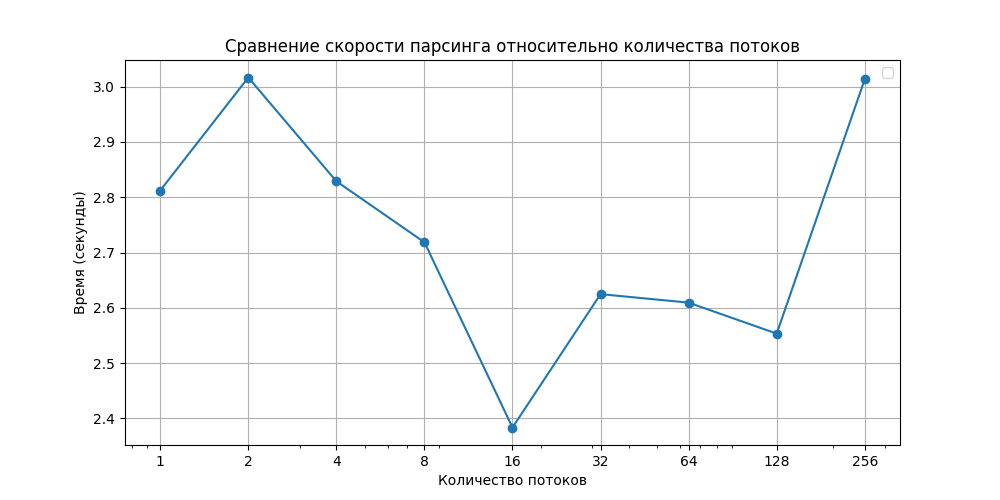
\includegraphics[scale=0.6]{inc/img/graph1.png}
    \caption{Зависимость времени выполнения программы от количества потоков}
    \label{fig:graph1}
\end{figure}
\clearpage


\section*{Вывод}
Параллельная обработка ускоряет выполнение программы по сравнению с последовательной версией~\cite{albahari_threading}. Время выполнения уменьшалось с увеличением числа потоков, но после определённого количества потоков улучшения производительности становились менее заметными. 
Время выполнения при использовании одного потока составило 2.81 секунды, в то время как при 16 потоках -- 2.38 секунды, что указывает на сокращение времени выполнения на примерно 15\%. Однако, при увеличении числа потоков с 16 до 128, улучшения в производительности были минимальными. Программа показывает наилучшую производительность при использовании 16 потоков, а наихудшую при использовании 2 и 256 потоков. При уменьшении числа потоков до 16 или 32 наблюдается заметное снижение эффективности работы.
Таким образом, эффективность параллельной обработки ограничена и зависит от множества факторов, таких как производительность устройства и особенности задачи.
\clearpage

\aaunnumberedsection{ЗАКЛЮЧЕНИЕ}{sec:outro}

Цель работы достигнута. В ходе выполнения данной лабораторной работы решены следующие задачи:
\begin{itemize}
    \item исследованы особенности предметной области и установлены критерии для оптимизации алгоритмов;
    \item разработаны два алгоритма для обработки данных: один для последовательной обработки, второй — с использованием параллельных потоков;
    \item проведено тестирование разработанных алгоритмов с оценкой их эффективности по временным затратам и использованию памяти;
    \item подготовлены графики и таблицы, демонстрирующие результаты сравнительного анализа производительности алгоритмов;
    \item в отчёте представлены полученные результаты о выполненной лабораторной работе.
\end{itemize}

Исследования показали, что использование параллельных потоков значительно ускоряет выполнение программы, особенно при увеличении количества потоков. Однако после достижения определённого числа потоков улучшения производительности становятся менее заметными, что связано с ограничениями устройства и особенностями решаемой задачи. Результаты исследования подтвердили эффективность параллельной обработки данных, при этом оптимальное количество потоков зависит от характеристик конкретной системы.
